%!TEX root = ../../../adrien_gomar_phd.tex
\chapter{Introduction to aeroelasticity}
\label{cha:ael}

\chabstract{In this chapter, the basic elements
to understand aeroelasticity in turbomachinery and by extension
in CROR are detailed. Firstly, the
definition and the basic equations that drive dynamic
aeroelasticity are presented. The two principal aeroelastic
phenomena that develop in turbomachinery are then presented.
The flutter is assessed in this thesis and the computational
approach retained to compute it, namely the weak-coupling approach,
is presented. The variables that are used to quantify the 
flutter boundary are finally presented.}


\newpage

\section{What is aeroelasticity}
\label{sec:what_is_ael}
%!TEX root = ../../../adrien_gomar_phd.tex

The study of aeroelasticity in turbomachineries takes its origin
in the first engines failure during the sixties~\cite{Dugundji2003}.
Also called dynamic aeroelasticity,
it is the interaction between three forces:
the aerodynamic ($\mathcal{A}$), the elastic ($\mathcal{E}$) and
the inertial forces ($\mathcal{I}$) as 
shown by the \citet{Collar1946} triangle represented in 
Fig.~\ref{fig:ael_collar_triangle}. 
\begin{figure}[htp]
  \centering
  \includegraphics*[width=0.40\textwidth]{collar_triangle.pdf}
  \caption{Collar triangle.}
  \label{fig:ael_collar_triangle}
\end{figure}

From a structural point of view, 
the dynamic aeroelasticity is governed by:
\begin{equation}
	M \ddot{x}(t) + D \dot{x}(t) + K x(t) = f(t)
	\label{eq:ael_motion_eq}
\end{equation}
where $M$, $D$ and $K$ are the structural mass, damping 
and stiffness matrices, respectively.
$x(t)$ and $f(t)$ denote the displacement 
and aerodynamic force vectors, respectively. The displacement
vector is defined relatively to the 
steady state position of the system. In turbomachinery
and by extension in CRORs, it is the steady state position
in rotation.


\section{Main aeroelastic phenomena in turbomachinery}
\label{sec:ael_phenomena}
%!TEX root = ../../../adrien_gomar_phd.tex

\subsection{Forced response}
\label{sub:forced_response}

As shown previously in Sec.~\ref{sec:cror_unsteady}, wakes and
potentials effects give rise to unsteady fluctuations in 
CROR configurations. These fluctuations 
can generate large vibration levels on the blades.
When the assembly modes are excited by the rotation speed
or its multiples, resonance can occur,
hence the term forced response. 
The frequency associated to the rotation speed or its multiples
is called Engine Order (EO).
At design, one step to minimize forced response is
to use the Campbell diagram show in Fig.~\ref{fig:campbell}
which schematically represents such resonance.
Blue points shows the crossing of engine order and 
the blade eigenfrequencies within the operating range. 
The Campbell diagram does not give any information of
the absolution level of vibration. Therefore, it is mostly
used to rank potential designs~\cite{Marshall1996}. This phenomena
will not be studied in this thesis.
\begin{figure}[htp]
  \centering
  \includegraphics*[width=0.40\textwidth]{campbell.pdf}
  \caption{Campbell diagram with forced response (blue circles)
  and flutter behavior (red stars).}
  \label{fig:campbell}
\end{figure}


\subsection{Flutter}
\label{sub:flutter}

Flutter is defined as a self-excited, unstable 
self-sustained vibration. In turbomachinery, this is
more likely to appear on blades.
One of the most impressive
manifestation of flutter occurred November 7\textsuperscript{th}, 1940.
Four month after being build, the bridge experienced 
torsional flutter excited by a $64$ \mbox{km/h} wind.
The first and second torsional modes were observed.
A few hours latter, the bridge felt down as seen in 
Fig.~\ref{fig:tacoma_bridge}. Hopefully, no human
was injured, but this event showed the importance
of taking into account the flutter phenomenon as
it is a very energetic event and can lead to the destruction of the system.
\begin{figure}[htp]
  \centering
  \subfigure[Torsion mode]{
      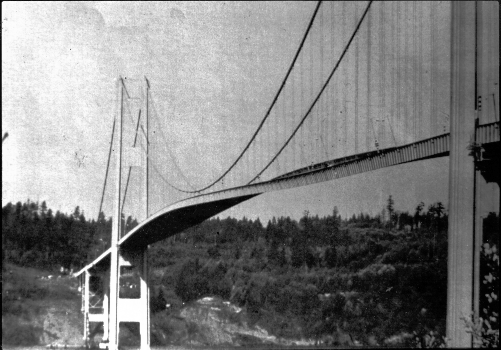
\includegraphics[height=.3\textwidth]{tac06.png}}
  \subfigure[Failure of the bridge]{
      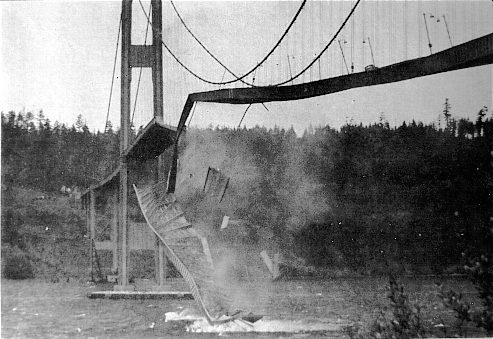
\includegraphics[height=.3\textwidth]{tac09.png}}
  \caption{Tacoma Narrows bridge flutter, from \citet{Smith1974}.}
  \label{fig:tacoma_bridge}
\end{figure}

Three vibration scenarios can appear, one leading to flutter.
The first scenario is the damped (or positively damped) 
vibration meaning
that the amplitude of the vibration decreases with respect to time, 
as shown in Fig.~\ref{fig:flutter_damped}.
This is the most wanted behavior as the system tends to
a stable point. In this case, the blade is said to
be flutter-free for the studied mode.
The second scenario is the amplified (or negatively damped)
vibration, namely flutter, shown in Fig.~\ref{fig:flutter_amplified}. 
This was the scenario that occurred on the Tacoma bridge. 
This scenario ultimately
leads to failure which is not acceptable. This is particularly true
on CROR configuration, as a blade failure might lead to 
the crash of the airplane as detailed in Sec.~\ref{sec:cror_challenges}.
The last scenario is the Limit Cycle Oscillation (LCO) vibration.
In this scenario, the deformation increases until a certain 
amplitude and then stays constant. This scenario is not
destructive by essence compared to the amplified scenario. However,
if the blade is repetitively excited by LCO, the blade
can fail as a consequence of structure fatigue.
\begin{figure}[htp]
  \centering
  \subfigure[damped (stable)]{
      \label{fig:flutter_damped}
      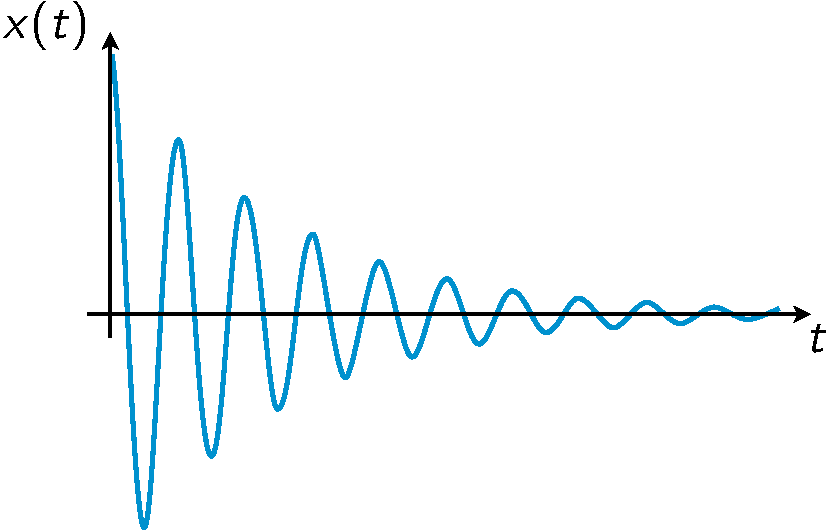
\includegraphics[width=.3\textwidth]{flutter_damped.pdf}}
  \subfigure[amplified (flutter)]{
      \label{fig:flutter_amplified}
      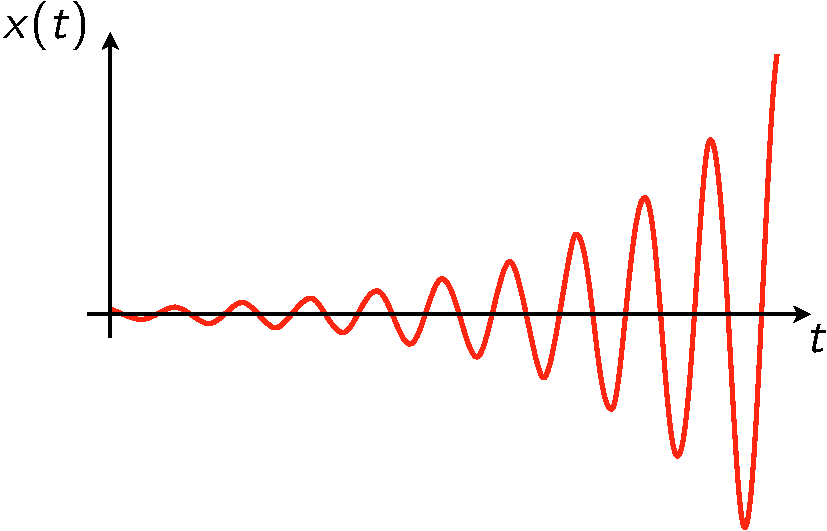
\includegraphics[width=.3\textwidth]{flutter_amplified.pdf}}
  \subfigure[Limit cycle oscillation]{
      \label{fig:LCO}
      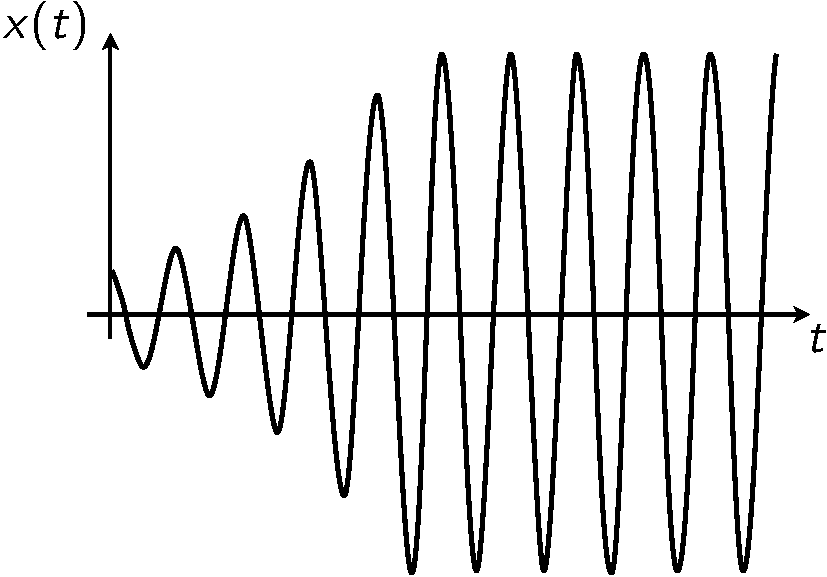
\includegraphics[width=.3\textwidth]{LCO.pdf}}
  \caption{Different vibration scenario for the flutter phenomenon.}
\end{figure}

The development of one scenario over another one is linked to
the fluid response to the vibration of the blade. In fact,
if the aerodynamic loads projected on the direction of the vibration
is positive, this means that the displacement will be amplified. 
In opposite, if the force is in opposed direction, the vibration will be damped.
The out-of-phase component of the aerodynamic force compared to
the displacement vector will give finally the sign of the aerodynamic damping.
The amplitude will give its strength. 

In this thesis, only the flutter boundary is assessed. In fact,
LCO can only be computed using a strong coupled fluid-structure 
approach and a weak coupling approach is chosen in this thesis
as detailed in the following Section.


\section{\texorpdfstring{\underline{C}}{C}omputational 
\texorpdfstring{\underline{A}}{A}ero\texorpdfstring{\underline{E}}{E}lasticity (CAE)}
\label{sec:cae}
%!TEX root = ../../../adrien_gomar_phd.tex

Solving this equation analytically is generally 
not feasible. In fact, in turbomachinery, 
the flow exhibits non-linear features such as turbulence, shock and
boundary-layer interaction, to name but a few, that are out of reach for
analytical methods.

Two main strategies exist then for solving equation~\ref{eq:ael_motion_eq}:
the strong-coupling and the weak-coupling. The strong-coupling 
approach solves either the equation directly or two solvers are coupled and 
compute the aerodynamic and structural response of the system, respectively.
The strong coupling remains computationally expensive~\cite{Bartels2007}
and numerically stiff~\cite{Datta2008}.
It is therefore not used in this thesis.

In opposite, the weak-coupling approach has been widely used
in the turbomachinery aeroelasticity community~\cite{Marshall1996}.
This method uses a modal approach to identify the structural modes.
This modes are then prescribed with an harmonic motion in the aerodynamic
flow solver and the damping is computed.

To do so the aerodynamic force $F(t)$ and
the structural damping matrix $D$ are considered to be zero
and Eq.~\eqref{eq:ael_motion_eq} becomes:
\begin{equation}
	M \ddot{x}(t) + K x(t) = 0.
	\label{eq:ael_motion_eq_free_response}
\end{equation}
Considering now that the displacement vector $x(t)$ is harmonic
yields the eigen-value problem:
\begin{equation}
	\mdet \left(K - \omega^2 M  \right) = 0.
	\label{eq:ael_motion_eq_eigen_value}
\end{equation}
The solution of this equation are the modes $\psi_r$
and their frequency $\omega_r$, verifying:
\begin{equation}
	\left(K - \omega_r^2 M  \right) \psi_r = 0.
\end{equation}
The modes define a modal basis 
$\Psi = [\psi_0, \psi_1, \dots \psi_n]$.
Once the modal basis
is identified, either by mean of a Finite
Element model or an experimental identification, 
equation~\ref{eq:ael_motion_eq} becomes:
\begin{equation}
  \label{eq:2}
  M_m \ddot{q}(t) + D_m \dot{q}(t) + K_m q (t) - \Psi^\top F(t)=0, \quad x(t) = \Psi q(t).
\end{equation}
$M_m$, $D_m$ and $K_m$ are the modal mass, 
damping and stiffness, respectively.
The weak coupling approach assumes the linearity of the response of
the fluid with respect to the displacement of the structure. Therefore
small displacements are assumed and the so-called Generalized
Aerodynamic Forces (GAF) are linearized, which adds aerodynamic
stiffness~$K_A$ and damping~$D_A$:
\begin{equation}
  \label{eq:4}
  \Psi^\top F(t) = D_A\dot{q}(t) + K_A q(t).
\end{equation}
In order to estimate the unsteady aerodynamic forces $F(t)$, 
a fluid simulation is run with a prescribed harmonic motion of the
structure:
\begin{equation}
  \label{eq:6}
  q(t)=\cos(\omega t).
\end{equation}
A stability analysis is then performed in the frequency domain:
\begin{equation}
  \label{eq:5}
  q=\hat{q}e^{p t}\Rightarrow\left(
    p^2M + p(D-D_A) + (K-K_A)
  \right)\hat{q}=0,
\end{equation}
where the Laplace variable $p$ is of the form
$p=i\omega(1+i\alpha)$. Finally, considering only weakly damped or
amplified modes (i.e. $|\alpha| \ll 1$), the damping of the
fluid/structure coupled system reads $\alpha=-\Re e(p)/\Im m(p)$.

\subsection{Structural dynamics of turbomachinery blade}
\label{sub:structural_dynamics_of_turbomachinery_blade}

The modes are classified by their global shape: 
bending/flexion (noted F) and torsion (noted T) 
modes are the main ones. Then they are classified
depending on the number of deflection lines that they
have. If one deflection line is present in a flexion 
mode, it is called 1F and 2F if two deflection lines are
seen, as shown in Fig.~\ref{fig:blade_mode_shape}.
\begin{figure}[htp]
  \centering
  \includegraphics*[width=0.40\textwidth]{blade_mode_shape.pdf}
  \caption{Blade mode shape nomenclature.}
  \label{fig:blade_mode_shape}
\end{figure}




